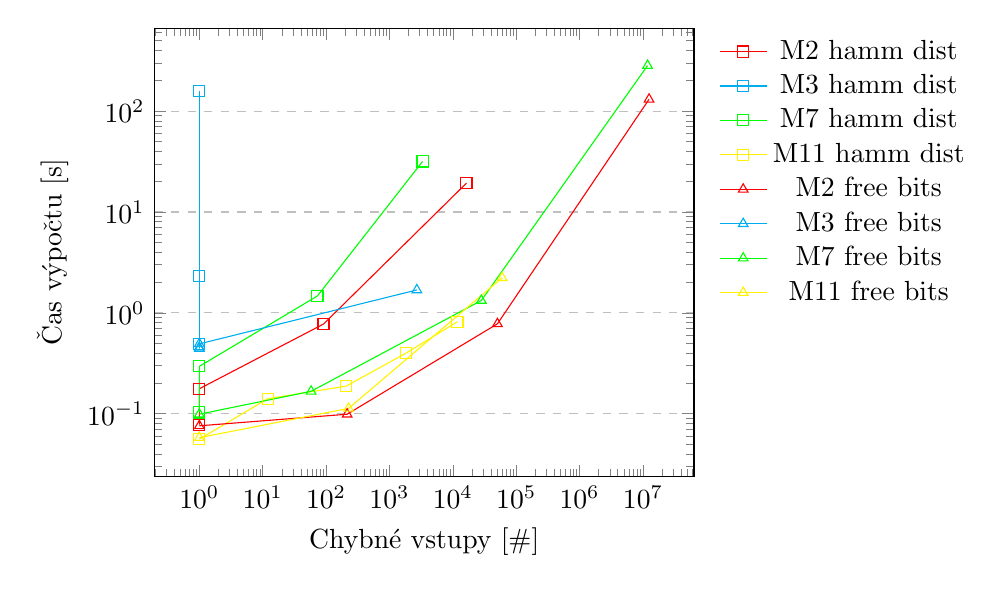
\begin{tikzpicture}
\begin{loglogaxis}[
    xlabel={Chybné vstupy [\#]},
    ylabel={Čas výpočtu [s]},
    legend pos=outer north east,
    legend style={draw=none, fill=none},
    ymajorgrids=true,
    grid style=dashed,
]

\addplot[
    color=red,
    mark=square,
    ]
    coordinates {
		(1, 0.078) (1, 0.177) (91, 0.775) (16404,19.316)
    };

\addplot[
    color=cyan,
    mark=square,
    ]
    coordinates {
		(1, 0.494) (1, 2.316) (1, 156.865)
    };

\addplot[
    color=green,
    mark=square,
    ]
    coordinates {
		(1, 0.103) (1, 0.295) (73, 1.471) (3330, 31.686)
    };

\addplot[
    color=yellow,
    mark=square,
    ]
    coordinates {
		(1, 0.056) (12, 0.141) (207, 0.188) (1813, 0.398) (11830, 0.818)
    };

\addplot[
    color=red,
    mark=triangle,
    ]
    coordinates {
		(1, 0.076) (215, 0.099) (50517, 0.779) (12467600, 130.907)
    };

\addplot[
    color=cyan,
    mark=triangle,
    ]
    coordinates {
		(1, 0.443) (1, 0.455) (1, 0.493) (2704, 1.688)
    };

\addplot[
    color=green,
    mark=triangle,
    ]
    coordinates {
		(1, 0.099) (58, 0.167) (28187, 1.327) (11819735, 282.620)
    };

\addplot[
    color=yellow,
    mark=triangle,
    ]
    coordinates {
		(1, 0.058) (226, 0.113) (60144, 2.229)
    };

\legend{M2 hamm dist, M3 hamm dist, M7 hamm dist, M11 hamm dist,
		M2 free bits, M3 free bits, M7 free bits, M11 free bits}

\end{loglogaxis}
\end{tikzpicture}
